\subsection{TOC-Based Simulation
Model}\label{toc-based-simulation-model}

The first step in developing the TOC-based simulation model was to
identify the constraint, or the drum of the DBR (\colorbox{yellow!40}{cf., Reference}).
Using the data from \colorbox{yellow!40}{}\hyperref[_Ref187517135]{Table 1}, along with
Tables S1 and S2 in the supplementary material, and assuming
\(p = \mathrm{\Delta}\varphi = 168\) hours, it was confirmed that
resource nine was the system's constraint, as it had the highest load
(i.e., \(l_{9} = 0.99\)), according to Equation 9. Consequently, the
positions of the CB and SB was set, as outlined in
\colorbox{yellow!40}{\hyperref[_Ref187516873]{Figure 2}}.

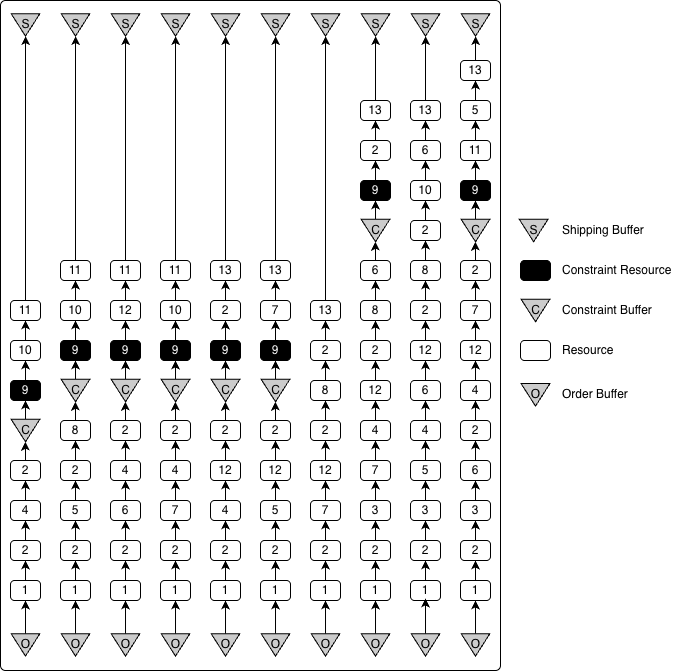
\includegraphics[width=4.64097in,height=4.53913in]{figures/fig02.png}

\protect\phantomsection\label{_Ref187516873}{}\colorbox{yellow!40}{Figure 2. Outline of
the reference model by Atwater and Chakravorty (2002).}

The implementation of the DBR rope considered three aspects, as
illustrated in \colorbox{yellow!40}{\hyperref[_Ref187516903]{Figure 3}}: (i) order
creation; (ii) scheduling; and (iii) order release. Order creation takes
place at the start of the order planning interval
\(\mathrm{\Delta}\varphi\), which in this case is \colorbox{yellow!40}{168 hours}. The
order size \(\left( M_{i}^{\mathrm{\Delta}\varphi} \right)\) is
calculated by Equation 17 and determines the reference level of the OB
for the order planning interval, i.e.,
\(\mathcal{b'}_{i}^{OB} = M_{i}^{\mathrm{\Delta}\varphi}\). Order
scheduling is modeled by Equation 15, which considers the throughput
\(\tau_{i}\) and the priority level of finished products in the SB
\(\left( \frac{\mathcal{b'}_{i}^{SB}}{H_{i}^{SB}} \right)\) (\colorbox{yellow!40}{cf.,
Reference}). In this context, we assume
\(\left( \rho_{i} - c_{i} \right) = 1\) when defining \(\tau_{i}\) in
the Equation 10, as the original work by Atwater and Chakravorty
(\colorbox{yellow!40}{2002}) does not consider the revenue and variable cost of each
product. Finally, order release, represented by
\(M_{i}^{\mathrm{\Delta}t}\), considers the consumption of the CB
\(\left( \mathcal{b'}_{i}^{CB} - H_{i}^{CB} \right)\) and the
work-in-process at each resource up to the constraint \(W_{i}^{CB}\)
(\colorbox{yellow!40}{cf., Reference}), as defined in Equation 19. The number of orders
released moderates the current level of the OB, denoted as
\(H_{i}^{OB}\).

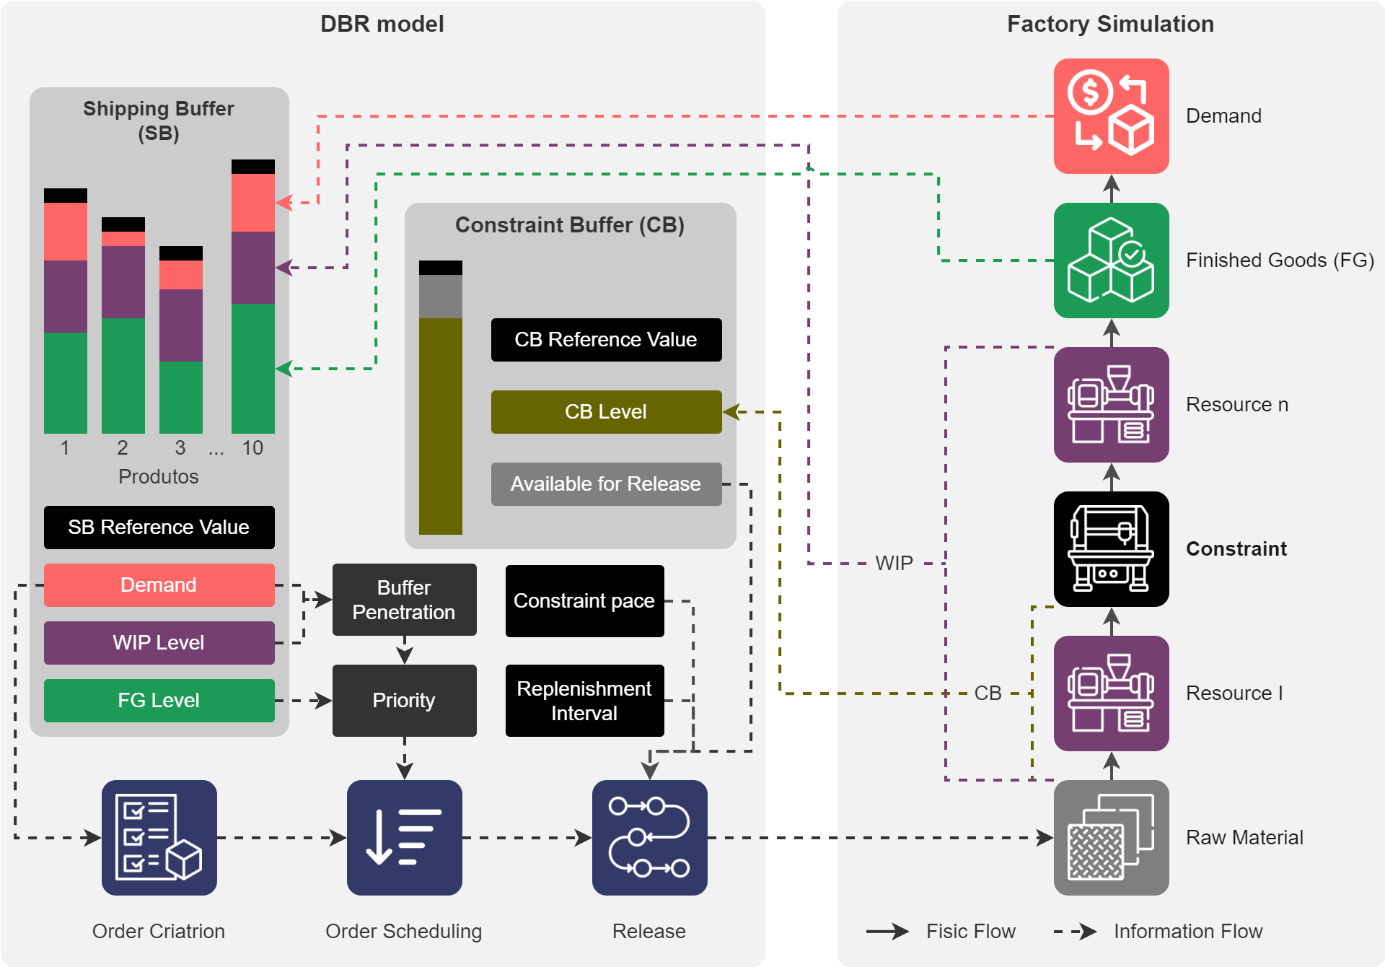
\includegraphics[width=6.29514in,height=4.39341in,alt={Diagrama Descrição gerada automaticamente}]{figures/fig03.png}

\protect\phantomsection\label{_Ref187516903}{}\colorbox{yellow!40}{Figure 3. Outline of
the TOC-based simulation model.}

The reference levels of the shipping buffers (SB) were calibrated with
the buffer-management (BM) policy described in Section 2.2. Fifteen
independent replications were run, each for 5,000,000 time units,
starting from a common oversized SB target. BM adjustments were held off
for the first 100,000 time units and then applied. For each product, the
SB target was aligned on a common time grid and averaged across
replications (Figure 4). The replication-average trajectories were
inspected graphically to identify the onset of steady state (Law, 2015).
From time 2,000,000 onward, the mean target of each replication was
computed and then averaged over the 15 replications; those values, after
rounding, were used as the fixed SB reference levels in the subsequent
experiments.

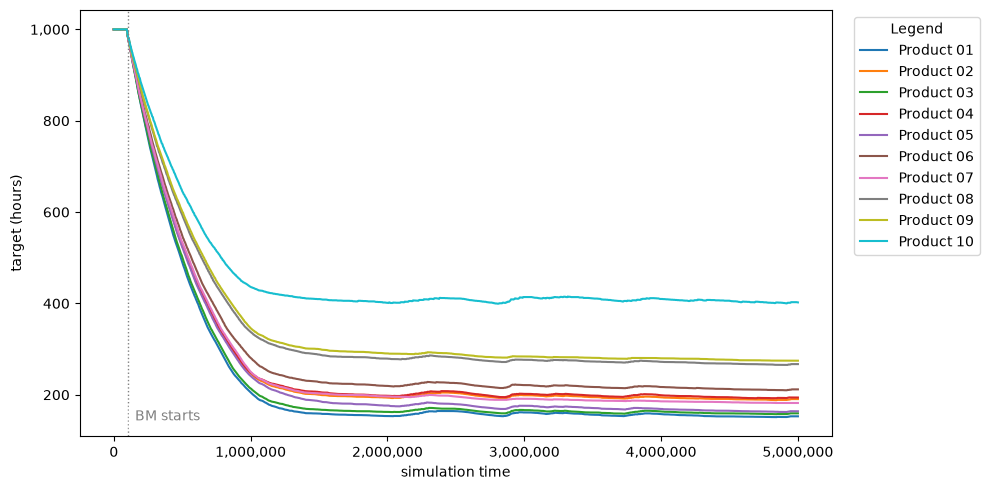
\includegraphics[width=6.29514in,height=3.12222in]{figures/fig04.png}

\colorbox{yellow!40}{Figure 4. Optimization of shipping buffer (SB) reference levels.}

The final reference level for each product in each buffer
\(\left( \mathcal{b'}_{i}^{x} \right)\), measured in terms of quantity
of semi-finished or finished products, is presented in
\hyperref[_Ref187517181]{Table 2}. These reference levels remained
constant throughout the experiments conducted in Section 5.

Table 2. Final reference leves for the shipping buffer (SB)

{\def\LTcaptype{none} % do not increment counter
\begin{longtable}[]{@{}
  >{\raggedright\arraybackslash}p{(\linewidth - 2\tabcolsep) * \real{0.3012}}
  >{\raggedright\arraybackslash}p{(\linewidth - 2\tabcolsep) * \real{0.1806}}@{}}
\toprule\noalign{}
\begin{minipage}[b]{\linewidth}\raggedright
Product \(i\)
\end{minipage} & \begin{minipage}[b]{\linewidth}\raggedright
\[\mathcal{b'}_{i}^{SB}\]
\end{minipage} \\
\midrule\noalign{}
\endhead
\bottomrule\noalign{}
\endlastfoot
1 & \colorbox{yellow!40}{0} \\
2 & \colorbox{yellow!40}{0} \\
3 & \colorbox{yellow!40}{0} \\
4 & \colorbox{yellow!40}{0} \\
5 & \colorbox{yellow!40}{0} \\
6 & \colorbox{yellow!40}{0} \\
7 & \colorbox{yellow!40}{0} \\
8 & \colorbox{yellow!40}{0} \\
9 & \colorbox{yellow!40}{0} \\
10 & \colorbox{yellow!40}{0} \\
\end{longtable}
}

The constraint-buffer (CB) target level was defined from an experiment
with 12 levels (from 250 to 800 units, in 50-unit steps), each simulated
for 50 replications. The decision used metrics with adequate sample size
(95\% CI relative half-width ≤ 5\%) that also varied significantly with
CB size (Kruskal-Wallis, α = 0.05). The level 350 was selected because
it sustained the same throughput as larger buffers while requiring the
smallest inventory, as presented on table 3.

\protect\phantomsection\label{_Ref187517181}{}Table 3. Metrics
comparison between constraint buffer (CB) target level.

{\def\LTcaptype{none} % do not increment counter
\begin{longtable}[]{@{}
  >{\raggedright\arraybackslash}p{(\linewidth - 4\tabcolsep) * \real{0.3015}}
  >{\raggedright\arraybackslash}p{(\linewidth - 4\tabcolsep) * \real{0.1686}}
  >{\raggedright\arraybackslash}p{(\linewidth - 4\tabcolsep) * \real{0.1808}}@{}}
\toprule\noalign{}
\begin{minipage}[b]{\linewidth}\raggedright
\[\mathcal{b'}_{i}^{CB}\]
\end{minipage} & \begin{minipage}[b]{\linewidth}\raggedright
\[\tau\]
\end{minipage} & \begin{minipage}[b]{\linewidth}\raggedright
\[i\]
\end{minipage} \\
\midrule\noalign{}
\endhead
\bottomrule\noalign{}
\endlastfoot
250 & \colorbox{yellow!40}{97,861} & \colorbox{yellow!40}{1,993} \\
300 & \colorbox{yellow!40}{99,884} & \colorbox{yellow!40}{2,082} \\
350 & \colorbox{yellow!40}{100,032} & \colorbox{yellow!40}{2,100} \\
400 & \colorbox{yellow!40}{100,036} & \colorbox{yellow!40}{2,105} \\
450 & \colorbox{yellow!40}{100,032} & \colorbox{yellow!40}{2,106} \\
500 & \colorbox{yellow!40}{100,036} & \colorbox{yellow!40}{2,108} \\
550 & \colorbox{yellow!40}{100,036} & \colorbox{yellow!40}{2,107} \\
600 & \colorbox{yellow!40}{100,037} & \colorbox{yellow!40}{2,109} \\
650 & \colorbox{yellow!40}{100,037} & \colorbox{yellow!40}{2,109} \\
700 & \colorbox{yellow!40}{100,036} & \colorbox{yellow!40}{2,109} \\
750 & \colorbox{yellow!40}{100,037} & \colorbox{yellow!40}{2,110} \\
800 & \colorbox{yellow!40}{100,037} & \colorbox{yellow!40}{2,110} \\
\end{longtable}
}
